%!TEX root = Main.tex
\section{Purpose}

To ensure that the scenario can be implemented to an existing system, it is important not to rewrite code of the existing system, but add to it, thus not breaking it for other developers.
The Common Ambient Assisted Living Homecare Platform, CAALHP, is a framework which behaves as a Context-Awareness system, just like the Java Context-Awareness Framework\cite{JCAF}, JCAF.
JCAF is built upon layers to ensure functionality and responsibility is divided to those who should handle it, allowing devices monitoring service by subscribing to them, letting services subscribe to devices and publish data to the monitors.
Another context framework implementing this technique is the Context Toolkit\cite{ContextToolkit}, which consist of several types of class, including \texttt{interpreters} to convert context to higher level information, and \texttt{discoverers} to register capabilities in the framework.

By using an object oriented model, a service for CAALHP (written in C\#) will be able to use inheritance, objects, an encapsulations to represent the data retrieved from the sensor and present them to monitors or other services, much as show on Figure \ref{fig:JCAF}.
The service will be automatically added to the CAALHP with context discoverers.

\begin{figure}[hbtp]
	\centering
	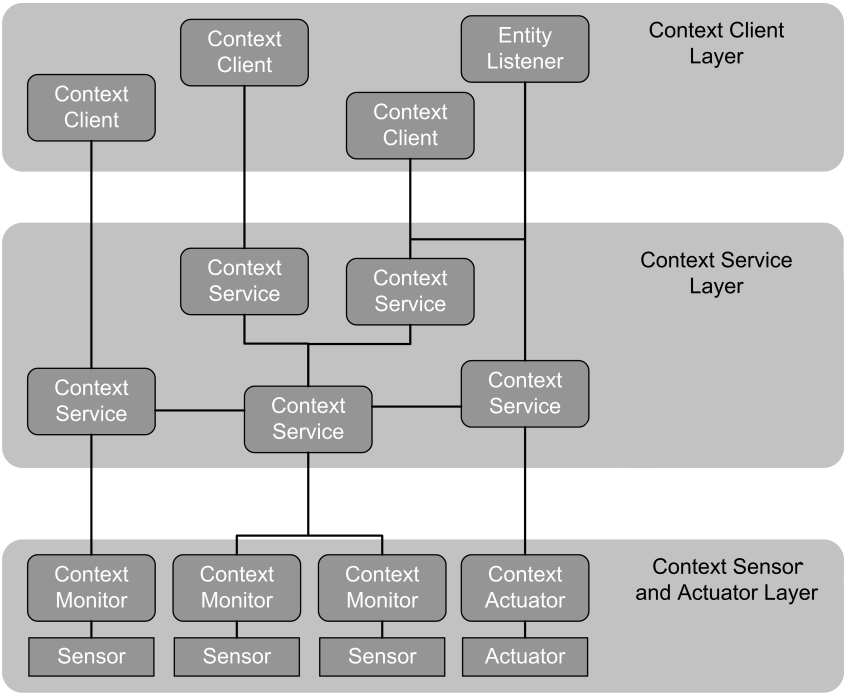
\includegraphics[width = 0.48 \textwidth]{JCAF}
	\caption{JCAF hierarchi\cite[5]{JCAF}. 
	Sensors are monitored by context monitors, which will provide the Context Service Layer with data from the sensors.
	The Context Services can subscribe to any number of Context Monitors and other Context Services, to calculate and present data for Context Clients, which can trigger alarms, display data for a user etc.}
	\label{fig:JCAF}
\end{figure}

The CAALHP is an Open Source project\cite{BB-CAALHP} which already operates with several different sensors and services.
Adding functionality must not affect other parts of the system -- it must run by it self, subscribing to the types of events coming into the system, and providing and API for the data the service handles.

